\thispagestyle{lichsutoanhocnone}
\pagestyle{lichsutoanhoc}
\graphicspath{{../lichsutoanhoc/pic/}}
\everymath{\color{lichsutoanhoc}}
\blfootnote{$^*$\color{lichsutoanhoc}Bài viết đăng tại https://mathshistory.st-andrews.ac.uk/Biographies/Galois/
}
\begingroup
\AddToShipoutPicture*{\put(0,616){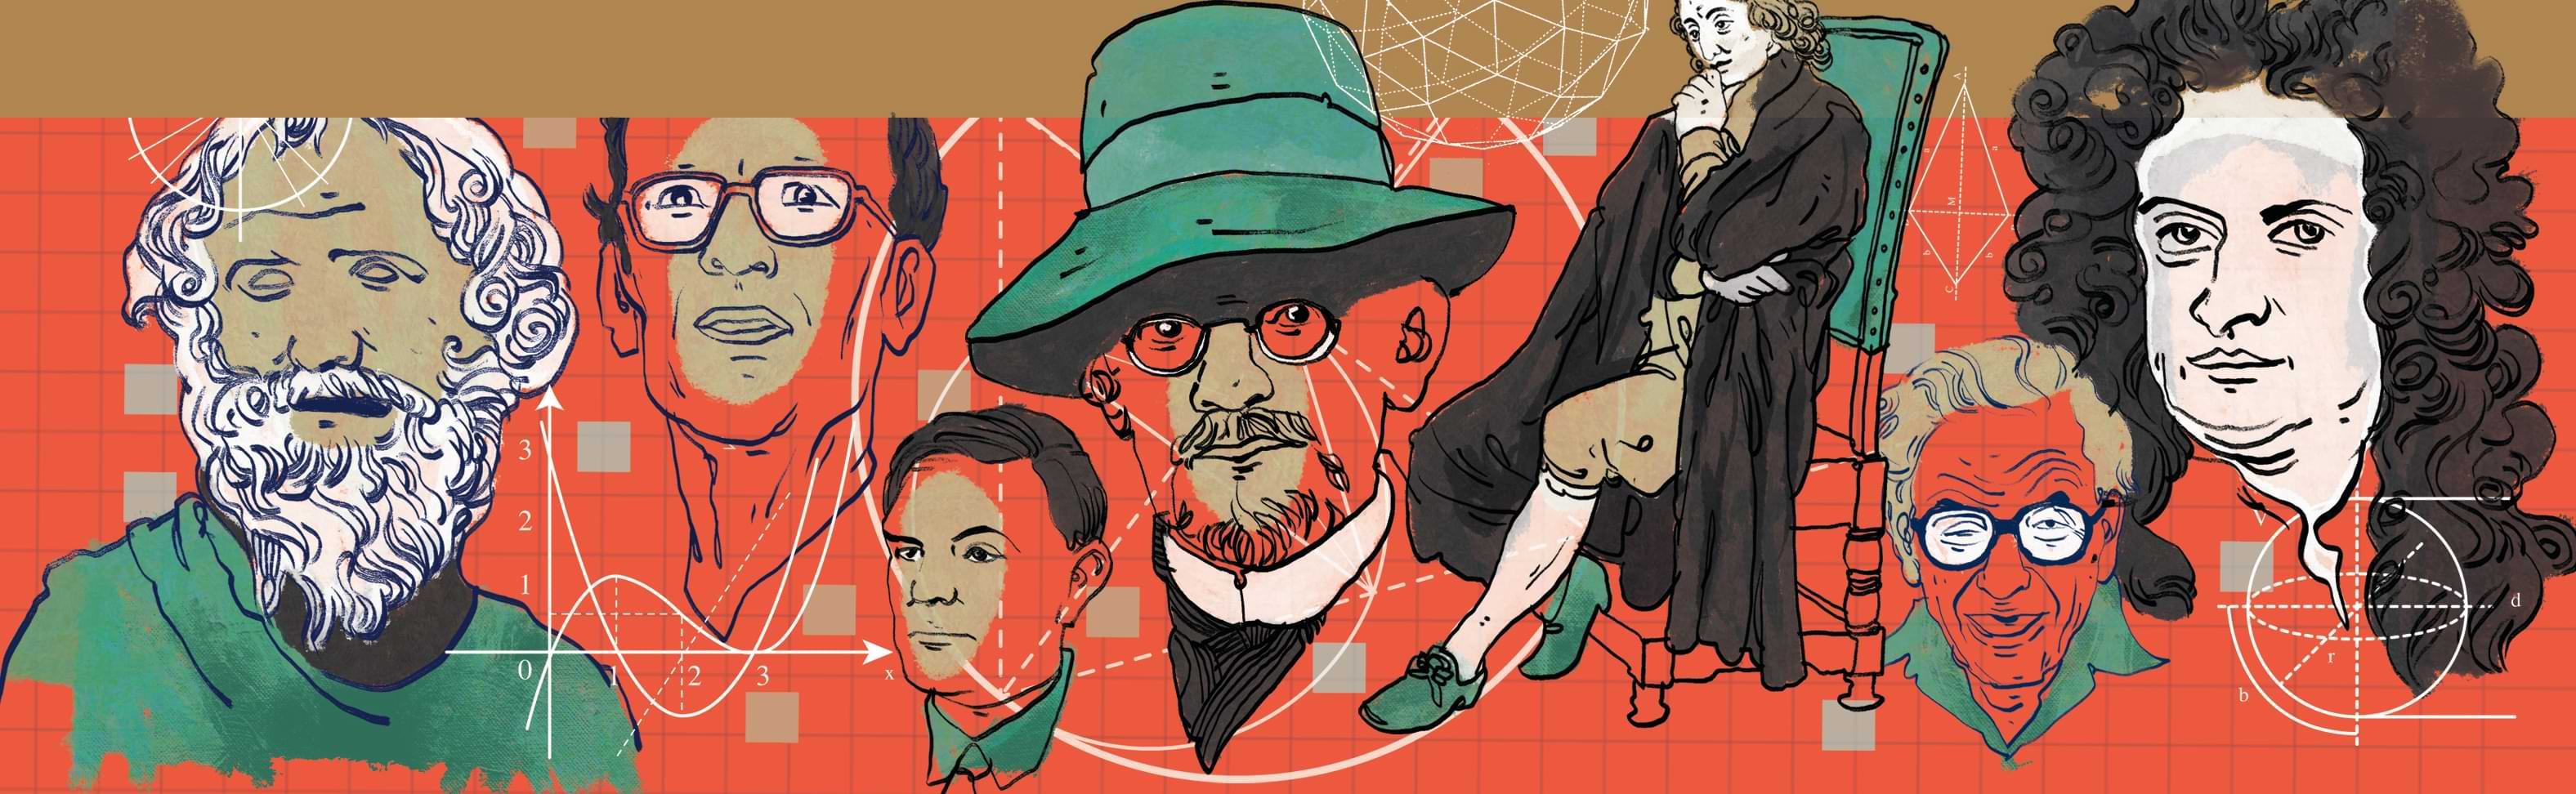
\includegraphics[width=19.3cm]{../bannerlichsu}}}
\AddToShipoutPicture*{\put(84,530){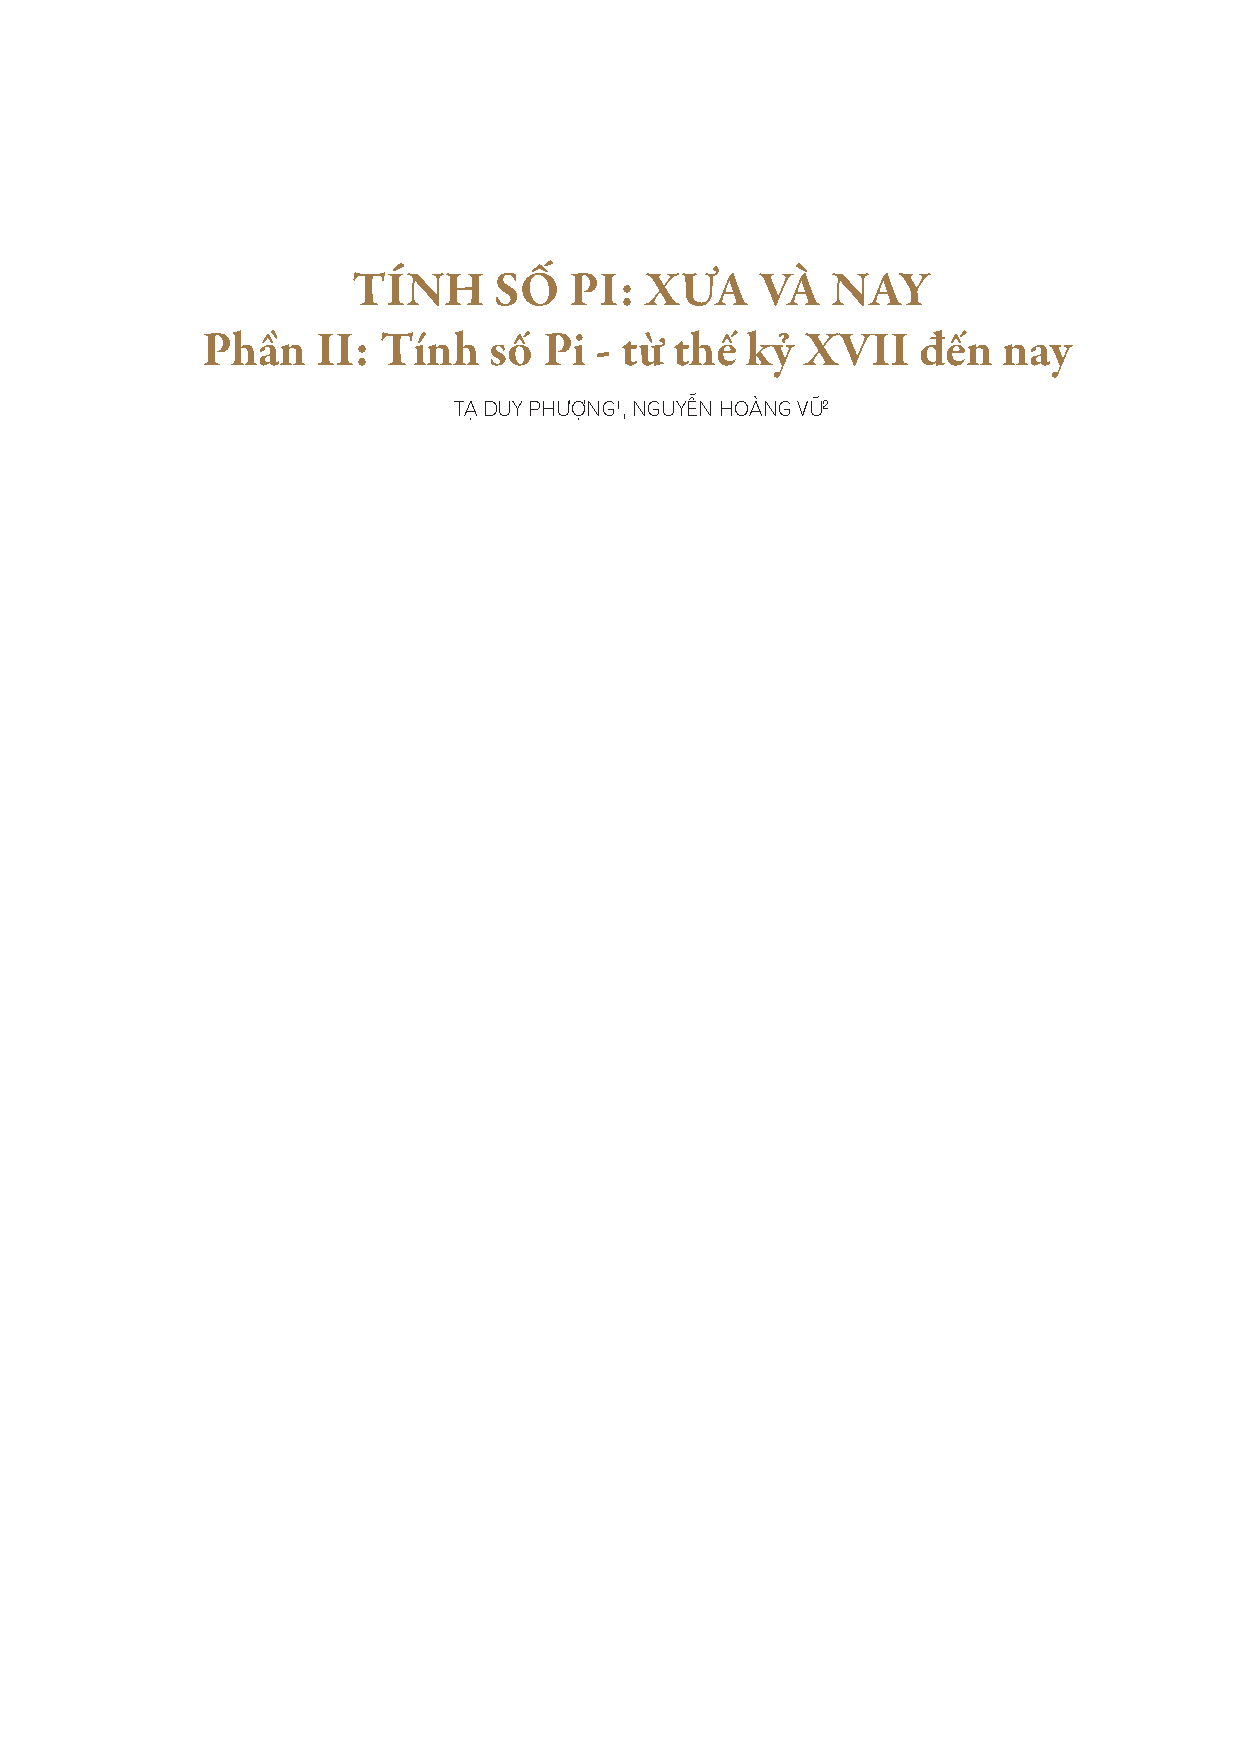
\includegraphics[scale=1]{../tieude.pdf}}}
\centering
\endgroup

\vspace*{180pt}

\begin{multicols}{2}
	\textit{Đi tới cội rễ của những tính toán này! Nhóm các phép toán lại! Phân loại chúng theo mức độ phức tạp hơn là vẻ ngoài của chúng! Điều đó, tôi tin rằng,  là sứ mệnh của các nhà toán học trong tương lai. Đó là con đường mà tôi đang dấn mình trong công việc này.}
	\begin{figure}[H]
		\vspace*{-5pt}
		\centering
		\captionsetup{labelformat= empty, justification=centering}
		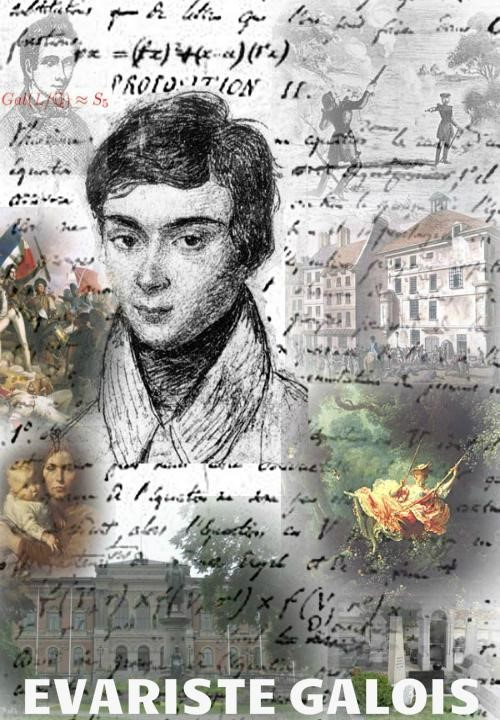
\includegraphics[width= 0.6\linewidth]{1}
		\caption{\small\textit{\color{lichsutoanhoc}Évariste Galois
				$(1811-1832).$}}
		\vspace*{-10pt}
	\end{figure}
	Cha của Évariste Galois là Nicholas Gabriel Galois và mẹ của anh là Adelaide Marie Demante đều là những người có trí tuệ và được đào tạo cẩn thận về triết học, văn học cổ điển và tôn giáo. Tuy nhiên không có một dấu hiệu nào về khả năng toán học trong số bất kỳ thành viên nào trong gia đình Galois. Mẹ của Galos là giáo viên duy nhất của anh cho đến khi anh $12$ tuổi. Bà dạy anh tiếng Hy Lạp, tiếng La--tin và tôn giáo, nơi bà truyền đạt sự hoài nghi của chính mình về nhà thờ cho con trai mình. Cha của Galois là một người quan trọng trong cộng đồng và năm 1815 ông được bầu làm thị trưởng xã Bourg--la--Reine.
	\begin{figure}[H]
		\vspace*{-5pt}
		\centering
		\captionsetup{labelformat= empty, justification=centering}
		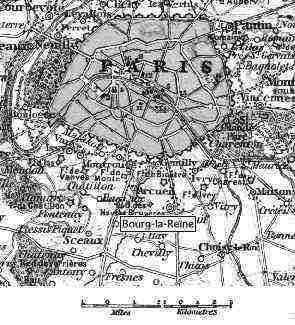
\includegraphics[width= 1\linewidth]{2}
		\caption{\small\textit{\color{lichsutoanhoc}Bản đồ Paris vào Thế kỷ $19$, có chỉ dẫn về xã Bourg--la--Reine.}}
		\vspace*{-10pt}
	\end{figure}
	Điểm khởi đầu của những sự kiện lịch sử đóng vai trò quan trọng trong cuộc đời Galois chắc chắn là Trận chiến  ngục Bastille nổ ra vào ngày $14$ tháng $7$ năm $1789$. Từ thời điểm này, chế độ quân chủ của Louis thứ $16$ gặp muôn vàn khó khăn khi phần lớn người dân nước Pháp gạt những cách biệt của họ để đoàn kết lại với nỗ lực đập tan hệ thống tổ chức đặc quyền của nhà thờ và nhà nước.
	\vskip 0.1cm
	Bất chấp những nỗ lực thỏa hiệp, Louis thứ $16$ vẫn bị xét xử sau khi cố gắng chạy trốn khỏi đất nước. Nối tiếp sau vụ hành quyết Nhà vua vào ngày $21$ tháng $1$ năm $1793$ là một Triều đại Khủng bố với nhiều vụ xét xử chính trị. Đến cuối năm $1793$ có $4595$ tù nhân chính trị bị giam giữ ở Paris. Tuy nhiên, nước Pháp bắt đầu có được những thời kỳ tốt đẹp hơn khi quân đội của họ, dưới sự chỉ huy của Napoléon Bonaparte, giành được hết  thắng lợi này đến  thắng lợi khác.
	\vskip 0.1cm
	Napoléon trở thành Tổng tài thứ nhất vào năm $1800$ và sau đó là Hoàng đế vào năm $1804$. Quân đội Pháp tiếp tục chinh phục châu Âu trong khi quyền lực của Napoléon ngày càng được đảm bảo. Vào năm $1811$, Napoléon đạt tới được đỉnh cao của quyền lực. Đến năm $1815$ thì sự cai trị của Napoléon đã khép lại. Theo sau Chiến dịch xâm lược nước Nga vào  năm $1812$ bị phá sản là những cuộc bại trận, quân Liên minh tiến vào Paris vào ngày $31$ tháng $3$ năm $1814$. Napoléon thoái vị vào ngày $6$ tháng $4$ và Louis XVIII được quân Liên minh phong làm Vua. Năm $1815$ đã chứng kiến Triều đại Một trăm ngày nổi tiếng. Napoléon tiến vào Paris ngày $20$ tháng $3$, bị đánh bại tại Waterloo vào ngày $18$ tháng $6$ và thoái vị lần thứ hai vào ngày $22$ tháng $6$. Louis XVIII được trở lại làm Vua nhưng qua đời vào tháng $9$ năm $1824$, Charles X trở thành Tân Vương.
	\vskip 0.1cm
	Vào thời gian đó Galois đang đi học ở trường. Cậu đã đăng ký học tại trường trung học  Louis--le--Grand với tư cách là học sinh nội trú lớp $4$ vào ngày $6$ tháng $10$ năm $1823$. Ngay trong học kỳ đầu tiên của cậu, đã xảy ra một cuộc nổi loạn nhỏ và $40$ học sinh đã bị đuổi khỏi trường. Galois không tham gia, và trong suốt năm học $1824-25$, thành tích học tập của cậu rất tốt và cậu đã nhận được một số giải thưởng. Tuy nhiên, vào năm $1826$, Galois bị yêu cầu học lại một năm vì bài hùng biện của cậu không đạt được tiêu chuẩn yêu cầu.
	\vskip 0.1cm
	Tháng 2 năm $1827$ là một bước ngoặt trong cuộc đời Galois. Anh đăng ký vào học lớp toán đầu tiên của mình, lớp của Hypolyte Vernier $(1800-1875)$. Anh  nhanh chóng đắm mình trong toán học và người Trưởng phòng đào tạo của Galois đã viết:
	\vskip 0.1cm
	\textit{Chính là niềm đam mê toán học đã chi phối cậu ấy, tôi nghĩ sẽ tốt nhất cho cậu ta nếu bố mẹ cậu không cho phép cậu ấy học gì ngoài môn này, cậu ta quả đang lãng phí thời gian ở đây và không làm gì khác ngoài việc hành hạ giáo viên và tự vùi lấp mình với những hình phạt.}
	\vskip 0.1cm
	Các bản học bạ ở trường của Galois bắt đầu mô tả anh là con người lập dị, kỳ quái, độc đáo và khép kín. Điều thú vị là có lẽ nhà toán học độc đáo nhất trong số những người từng sống lại bị than phiền vì tính cách độc đáo của mình. Tuy nhiên, Vernier đã báo cáo rằng:
	\vskip 0.1cm
	\textit{Có trí tuệ, tiến bộ rõ rệt nhưng chưa đủ phương pháp.}
	\vskip 0.1cm
	Năm $1828$ Galois thi vào École Polytechnique nhưng bị trượt. Đó là trường Đại học hàng đầu của Paris và Galois hẳn đã mong ước đỗ vào được trường này vì những lý do học thuật. Tuy nhiên, anh cũng mong muốn được vào trường này cả vì những phong trào chính trị mạnh mẽ tồn tại trong giới sinh viên của trường, vì Galois đã noi gương cha mẹ mình để trở thành một người theo Cộng hòa một cách nhiệt thành.
	\vskip 0.1cm
	Trở lại Louis--le--Grand, Galois đăng ký vào lớp toán của Louis Richard. Tuy nhiên, anh ngày càng làm việc nhiều hơn cho các nghiên cứu của riêng mình và ngày càng ít làm bài tập ở trường. Anh nghiên cứu cuốn Géométrie của Legendre và các chuyên luận của Lagrange. Như Richard đã từng thông báo lại:
	\vskip 0.1cm
	\textit{Sinh viên này chỉ có làm việc trong những lĩnh vực toán học cao nhất.}
	\vskip 0.1cm
	Vào tháng $4$ năm $1829$ Galois có bài báo toán học đầu tiên được xuất bản trên tạp chí Annales de mathématiques. Vào ngày $25$ tháng $5$ và ngày $1$ tháng $6$, anh đã gửi các bài báo về nghiệm đại số của phương trình tới Académie des Sciences. Cauchy được phân công làm phản biện cho bài báo của Galois.
	\vskip 0.1cm
	Một bi kịch ập đến với Galois bởi vào ngày $2$ tháng $7$ năm $1829$, cha anh đã tự sát. Vị linh mục của xã Bourg--la--Reine đã giả mạo tên của Thị trưởng Galois trên những bài thơ trào phúng hiểm độc bị làm giả nhằm vào chính những người họ hàng của Galois. Cha của Galois vốn là một người đàn ông hiền hậu, và vụ bê bối xảy ra sau đó đã khiến ông không thể chịu đựng nổi. Ông đã treo cổ tự tử trong căn hộ ở Paris, chỉ cách Louis--le--Grand nơi con trai ông đang học có vài bước chân. Galois bị ảnh hưởng sâu sắc bởi cái chết của cha mình, và điều đó đã ảnh hưởng rất lớn đến hướng đi của cuộc đời anh.
	\vskip 0.1cm
	Vài tuần sau cái chết của cha mình, Galois đã tự mình đến dự kỳ thi tuyển vào École Polytechnique lần thứ hai. Lần thứ hai anh thất bại, có lẽ một phần vì anh đã phải tham gia kỳ thi trong hoàn cảnh tồi tệ nhất có thể xảy ra ngay sau khi cha anh qua đời, một phần vì anh chưa bao giờ giỏi trong việc truyền đạt những ý tưởng toán học sâu sắc của mình. Do đó, Galois đã phải cam chịu để vào École Normale, một trường nằm sát với  Louis--le--Grand, và để làm được điều đó, anh phải tham gia kỳ thi Tú tài, điều mà anh đã có thể tránh được bằng cách thi vào École Polytechnique.
	\vskip 0.1cm
	Anh đã đỗ kì thi và nhận bằng vào ngày $29$ tháng $12$ năm $1829$. Người chấm thi môn toán của anh đã thông báo: 
	\vskip 0.1cm
	\textit{Cậu học trò này đôi khi còn mù mờ trong việc diễn đạt ý tưởng của mình nhưng lại có trí tuệ và thể hiện một tinh thần nghiên cứu đáng chú ý.}
	\vskip 0.1cm
	Người chấm thi môn văn học của anh đã thông báo: 
	\vskip 0.1cm
	\textit{Đây là học sinh duy nhất đã trả lời tôi rất kém, cậu ấy hoàn toàn không biết gì cả. Tôi được mọi người nói trước lại rằng cậu học sinh này có năng lực toán học phi thường. Điều này làm tôi vô cùng ngạc nhiên, vì sau khi kiểm tra, tôi tin rằng anh ta cũng có nhưng chỉ một chút ít trí tuệ.}
	\vskip 0.1cm
	Galois đã gửi cho Cauchy nghiên cứu tiếp theo về lý thuyết  các phương trình, nhưng sau đó anh đã tìm hiểu được từ Bulletin de Férussac về một bài báo để lại sau khi qua đời của Abel có phần đan xen với một phần nghiên cứu của anh. Sau đó Galois nghe theo lời khuyên của Cauchy và gửi đăng một bài báo mới \textit{Về  điều kiện để một phương trình có thể giải được bằng căn thức} vào tháng $2$ năm $1830$. Bài báo được gửi tới Fourier, thư ký của Viện Hàn lâm Paris, để được xét Giải thưởng lớn về toán học. Fourier qua đời vào tháng $4$ năm $1830$, và bài báo của Galois sau đó đã không bao giờ được tìm thấy, và do đó đã không bao giờ được xét giải.
	\vskip 0.1cm
	Sau khi đọc tác phẩm của Abel và Jacobi, Galois đã nghiên cứu lý thuyết về các hàm elliptic và các tích phân abelian. Với sự hỗ trợ từ Jacques Sturm, anh đã công bố ba bài báo trên Bulletin de Férussac vào tháng $4$ năm $1830$. Tuy nhiên, vào tháng $6$, anh được biết rằng giải thưởng của Học viện sẽ được trao chung cho Abel (sau khi qua đời) và cho Jacobi,  trong khi tác phẩm của anh lại  chưa hề được xét.
	\vskip 0.1cm
	Tháng $7$ năm $1830$ chứng kiến một cuộc Cách mạng. Charles thứ $10$ trốn khỏi nước Pháp. Bạo loạn nổ ra trên những đường phố của Paris, và vị hiệu trưởng của École Normale, ông M. Guigniault, đã khoá  các sinh viên lại  ở trong trường  để tránh không cho họ tham gia. Galois đã cố gắng trèo qua bức tường để tham gia cuộc bạo loạn, nhưng không thành công. Vào tháng $12$ năm $1830$ ông M. Guigniault đã viết các bài báo công kích sinh viên, và Galois đã viết bài trả lời trên Gazette des Écoles, phản kháng lại M. Guigniault vì những hành động khoá nhốt sinh viên trong trường của ông ta. Vì lá thư này, Galois đã bị đuổi học,  và anh gia nhập Pháo binh của Lực lượng Vệ binh Quốc gia, một chi nhánh của lực lượng dân quân thuộc nền Cộng hòa. Vào ngày $31$ tháng $12$ năm $1830$, Pháo binh Vệ binh Quốc gia bị phế bỏ theo Chiếu chỉ Hoàng gia vì vị Vua mới Louis--Phillipe cảm thấy lực lượng là mối đe dọa đối với ngai vàng.
	\vskip 0.1cm
	Hai ấn phẩm nhỏ, một bản tóm tắt trên Annales de Gergonne (tháng $12$ năm $1830$) và một trao đổi về giảng dạy khoa học trên Gazette des Écoles (ngày $2$ tháng $1$ năm $1831$) là những ấn phẩm cuối cùng trong cuộc đời anh. Vào tháng $1$ năm $1831$ Galois cố gắng quay trở lại với toán học. Anh tổ chức một số lớp  toán về đại số cao cấp, buổi đầu tiên thu hút $40$ học sinh nhưng sau đó con số này nhanh chóng sụt giảm. Galois được Poisson mời gửi phiên bản thứ ba của cuốn luận văn của anh về phương trình cho Viện hàn lâm và anh đã thực hiện điều này vào ngày $17$ tháng $1$.
	\vskip 0.1cm
	Vào ngày $18$ tháng $4$, Sophie Germain đã viết một lá thư cho một người  bạn của bà là nhà toán học Libri, mô tả hoàn cảnh của Galois:
	\vskip 0.1cm
	\textit{... cái chết của M. Fourier, là quá sức chịu đựng đối với cậu sinh viên Galois này, một người, bất chấp tính xấc xược của mình,  vẫn thể hiện những dấu hiệu của một tính cách thông minh. Tất cả những điều này đã ập đến nhiều đến mức cậu ta bị đuổi học khỏi École Normale. Cậu ta giờ không có tiền.... Họ nói cậu ta sẽ hoàn toàn phát điên. Tôi e sợ điều này lại là sự thật.}
	\vskip 0.1cm
	Cuối năm $1830$, $19$ sỹ quan thuộc Pháo binh của Vệ binh Quốc gia bị bắt và bị buộc tội âm mưu lật đổ chính phủ. Họ được trắng án và vào ngày $9$ tháng $5$ năm $1831$, $200$ người Cộng hòa đã tụ tập ăn tối để ăn mừng sự trắng án. Trong bữa tối, Galois nâng ly của mình và với một con dao găm để hở trong tay, anh có vẻ như đang nói những lời đe dọa chống lại Nhà vua, Louis--Phillipe. Sau bữa tối, Galois bị bắt và bị giam tại nhà tù Sainte--Pélagie. Tại phiên tòa xét xử vào ngày $15$ tháng $6$, luật sư bào chữa của anh ta khai rằng Galois đã nói:
	\vskip 0.1cm
	Dành cho Louis--Phillipe, nếu ông ta phản bội.
	\vskip 0.1cm
	nhưng những lời cuối cùng đã bị tiếng ồn nhấn chìm. 
	\vskip 0.1cm
	Galois, một cách khá ngạc nhiên do vẫn lặp lại chính những lời đe dọa đó từ bục xử án, đã được trắng án.
	\vskip 0.1cm
	Ngày $14$ tháng $7$ là Ngày Bastille và Galois lại bị bắt. Anh mặc đồng phục của Pháo binh Vệ binh Quốc gia, điều này là bất hợp pháp. Anh cũng mang theo một khẩu súng trường đã nạp đạn, một số khẩu súng lục và một con dao găm. Galois bị đưa trở lại nhà tù Sainte--Pélagie. Khi ở trong tù, anh nhận được lời từ chối với cuốn Luận văn của mình. Poisson đã thông báo rằng: 
	\vskip 0.1cm
	\textit{Lập luận của ông ấy chưa đủ rõ ràng, cũng như chưa được phát triển đầy đủ để cho phép chúng ta đánh giá tính chính xác của nó.}
	\vskip 0.1cm
	Tuy nhiên, ông đã khuyến khích Galois xuất bản một bản  trình bày đầy đủ hơn về công trình của mình. Khi ở trong nhà tù Sainte--Pélagie, Galois đã cố gắng tự vẫn bằng cách dùng dao găm đâm mình nhưng các tù nhân khác đã ngăn cản anh ta. Trong cơn say trong tù, anh đã trút hết tâm hồn mình:
	\vskip 0.1cm
	\textit{Bạn có biết tôi thiếu gì không, bạn tôi ơi? Tôi tâm sự điều đó chỉ với bạn: đó chính là người mà tôi có thể yêu và chỉ có thể yêu thương bằng tinh thần. Tôi đã mất cha và không ai có thể thay thế được ông, bạn có nghe thấy không...?}
	\vskip 0.1cm
	Vào tháng $3$ năm $1832$, một trận dịch tả càn quét Paris và các tù nhân, bao gồm cả Galois, được chuyển đến nhà dưỡng lão Sieur Faultrier. Ở đó, dường như anh  đã phải lòng Stephanie--Felice du Motel, con gái của một bác sĩ nội trú. Sau khi anh được thả vào ngày $29$ tháng $4$, Galois đã trao đổi thư từ với Stephanie, và rõ ràng là cô ấy đã cố gắng tránh xa mối quan hệ này.
	\begin{figure}[H]
		\vspace*{-5pt}
		\centering
		\captionsetup{labelformat= empty, justification=centering}
		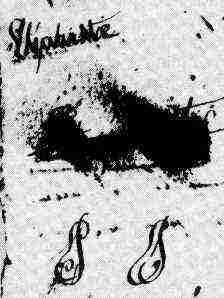
\includegraphics[width= 1\linewidth]{3}
		\caption{\small\textit{\color{lichsutoanhoc}Tên Stephanie xuất hiện trong một bản thảo của Galois.}}
		\vspace*{-10pt}
	\end{figure}
	Cái tên Stephanie xuất hiện nhiều lần ở phần ghi chú bên lề trong một trong những bản thảo của Galois. 
	\vskip 0.1cm
	Galois đã đấu súng với Perscheux d'Herbinville vào ngày $30$ tháng $5$, lý do của cuộc đấu súng này không ai biết, nhưng chắc chắn có liên quan đến Stephanie.
	\vskip 0.1cm
	Một ghi chú bên lề của bản thảo mà Galois đã viết vào đêm trước trận đấu súng nổ ra, có nội dung:
	\vskip 0.1cm
	\textit{Có một điều gì đó phải hoàn thành trong phép chứng minh này. Tôi không có thời gian. (Ghi chú của tác giả).}
	\vskip 0.1cm
	Chính điều này đã dẫn đến truyền thuyết rằng Galois đã dành cả đêm cuối cùng trong cuộc đời mình để viết ra tất cả những gì anh biết về lý thuyết nhóm. Nhưng câu chuyện này có vẻ dường như đã bị phóng đại.
	\begin{figure}[H]
		\vspace*{-5pt}
		\centering
		\captionsetup{labelformat= empty, justification=centering}
		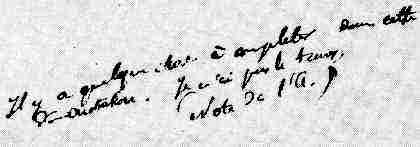
\includegraphics[width= 1\linewidth]{4}
		\caption{\small\textit{\color{lichsutoanhoc}Ghi chép bên lề của Galois.}}
		\vspace*{-10pt}
	\end{figure}
	Galois bị thương trong cuộc đấu súng và bị d'Herbinville cùng chính những người ``bạn" là những đại diện trung gian của anh bỏ rơi, và sau đó được một người nông dân tìm thấy. Anh qua đời tại bệnh viện Cochin vào ngày $31$ tháng $5$, và tang lễ của anh được tổ chức vào ngày $2$ tháng $6$. Đây là tâm điểm của một cuộc biểu tình của nền Cộng hòa và các cuộc bạo loạn kéo dài trong vài ngày.
	\vskip 0.1cm
	Anh trai của Galois và bạn của anh là Chevalier đã chép lại các bài báo toán học của anh và gửi cho Gauss, Jacobi và những người khác. Galois đã từng mong muốn được Jacobi và Gauss đưa ra những quan điểm của mình về công trình của anh. Không có ghi chép nào về bất kỳ bình luận của những người này đã đưa ra. Tuy nhiên, các bài báo đã đến tay Liouville, người vào tháng $9$ năm $1843$ đã thông báo với Học viện rằng ông đã tìm thấy trong các bài báo của Galois một lời giải ngắn gọn
	\vskip 0.1cm	
	\textit{...vừa chính xác vừa sâu sắc của bài toán đáng yêu này: Cho một phương trình bậc nguyên tố bất khả quy, hãy quyết định xem nó có giải được bởi các căn thức hay không.}
	\vskip 0.1cm
	Liouville đã xuất bản những bài viết này của Galois trong Tạp chí của ông vào năm $1846$.
	\vskip 0.1cm
	Lý thuyết mà Galois phác thảo ra những nét chính trong các bài báo này hiện nay được gọi là Lý thuyết Galois.
\end{multicols}